\documentclass[a4paper,11pt,titlepage]{article}
\usepackage[czech]{babel}
\usepackage[utf8]{inputenc}
\usepackage{rotating}
\usepackage{graphicx}
\pagestyle{headings}
\author{Radka Mokrá, Lukáš Brabec, Aleš Dujíček, Jan Sedlák}
\title{Dokumentace k projektu pro předměty IAL a IFJ}
\frenchspacing

\begin{document}
%\maketitle
\thispagestyle{empty}

\begin{center}
\Large{\scshape Vysoké učení technické v Brně}

\vspace{0.5cm}

\large{Fakulta informačních technologií}

\vfill

\Large{\scshape Dokumentace k projektu pro přeměty IAL a IFJ}

% \vspace{0.5cm}
%
% 2010/2011

\vfill

\LARGE{Překladač jazyka IFJ11}

\vfill

\large{Tým 097, varianta a/1/I}
\end{center}

\vspace{0.5cm}

\begin{tabular}{l l r l}
Radka Mokrá  & \tt{xmokra00} & 34\% & vedoucí \\ 
Lukáš Brabec & \tt{xbrabe09} &  0\% & \\
Aleš Dujíček & \tt{xdujic01} & 33\% & \\
Jan Sedlák   & \tt{xsedla85} & 33\% & \\
\end{tabular}

%\begin{flushright}
%\today
%\end{flushright}

\newpage{}


\tableofcontents

\newpage

\section{Úvod}
Tento text je dokumentací k týmovému projektu do kurzu IFJ (Formální jazyky a překladače) a IAL (Algoritmy). Popisuje implementaci interpretru jazyka inspirovaného programovacím jazykem Lua. Pro řešení byla vybrána varianta a/1/I, řazení je implementováno algoritmem quicksort, tabulka symbolů binárním stromem a vyhledávání podřetězců Knuth-Morris-Prat\-to\-vým algoritmem.

\section{Lexikální analýza}
Lexikální analyzátor je navržen a implementován jako deterministický ko\-neč\-ný automat, jehož graf přechodů je zobrazen na obrázku \ref{lex.lex}. Symbol \ae{} značí všechny ostatní symboly, pro které z daného stavu není jiný přechod.

\begin{figure}[h!]
\centering
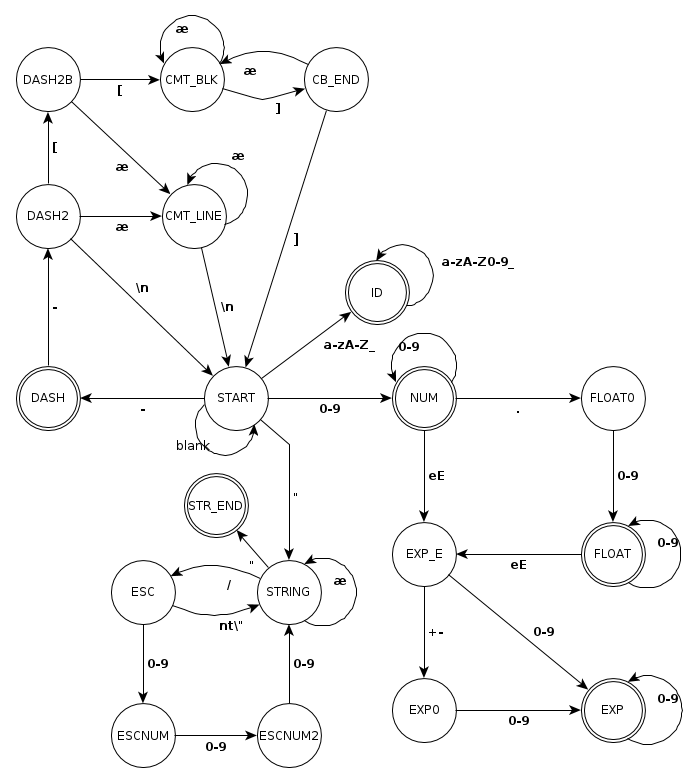
\includegraphics[width=11cm]{lexical.png}
\caption{Schéma konečného automatu lexikálního analyzátoru}
\label{lex.lex}
\end{figure}

V koncovém stavu pro indentifikátory skončí i klíčová a rezervovaná slova. Kdyby je měl automat zpracovávat zvlášť, přibylo by mnoho stavů a automat by se stal nepřehledným. Proto jsou zpracovány spolčně s identifikátory a na konci je volána funkce, která určí, zda se skutečně jedná o identifikátor, nebo některé z klíčových nebo rezervovaných slov.

Graf na obázku \ref{lex.lex} není úplný, zobrazuje jen analýzu řetězců, identifikátorů, čísel a komentářů. Analýza ostatních lexémů, jedná so o operátory, je realizována jen jedním, případně dvěma, přechody z počátečního stavu {\tt start}. Graf by se ale při takovém množství přechodů z počátečního stavu stal nepřehledným. Proto je jejich zpracování zobrazeno obrázku \ref{lex.ope} zvlášť od složitější a zajímavější části automatu.

\begin{figure}
\centering
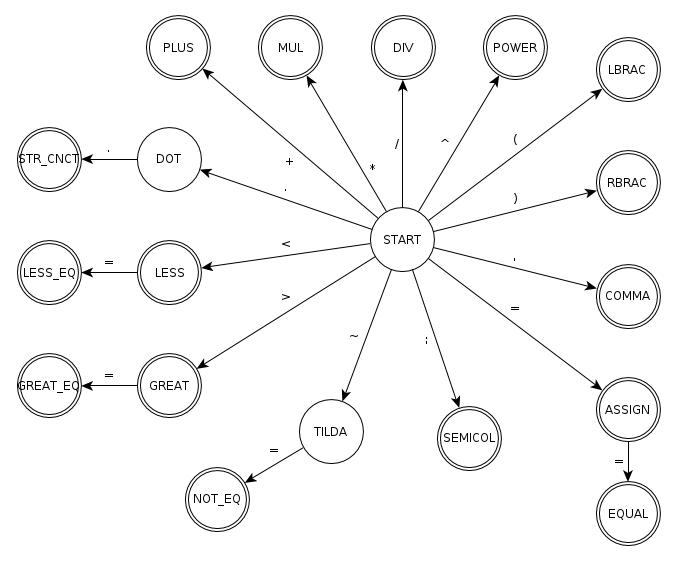
\includegraphics[width=10cm]{operator.png}
\caption{Schéma konečného automatu lexikálního analyzátoru}
\label{lex.ope}
\end{figure}


\section{Syntaktická analýza}

Syntaktická analýza je prováděna rekurzívním sestupem shora dolů. Vytvořili jsme proto bezkontextovou gramatiku, pro kterou jsou terminálními symboly tokeny, které vrací lexikální analyzátor. Neterminální symboly popisují jednotlivé konstrukce jazyka IFJ11. Tuto gramatiku jsme vytýkáním a odstraněním levé rekurze převedli na LL-gramatiku, jejíž pravidla jsou na obrázku \ref{syn.prog}.

Počátečním neterminálním symbolem je symbol {\tt program}. Každý neterminální symbol je v analyzátoru reprezentován funkcí, která zpracovává pravou stranu pravidla. Pokud je na pravé straně pravidla terminální symbol, je kontrolováno, zda lexikální analyzátor právě takový token načetl. Pokud ne, jedná se o syntaktickou chybu. Neterminální symboly na pravé straně vedou k volání funkce, která tento symbol reprezentuje.

Výrazy jsou zpracovávány metodou zdola nahoru a je jim věnována následující podkapitola.


\subsection{Analýza výrazů}
Analýza výrazů je obstarána funkcí {\tt expression()}, kterou zavolá parser, když je dle pravidel očekáván výraz. Výrazy jsou zpracovány pomocí precedenční syntaktické analýzy zdola nahoru, která je realizována zásobníkovým automatem. Pro tuto potřebu byla vytvořena precedenční tabulka zobrazená v tabulce \ref{tab.prec}, která určuje jak zásobníkový automat reaguje na vstupní token v závislosti na terminálním symbolu nejblíže vrcholu zásobníku. Gramatika popisující výrazy je uvedena na obrázku \ref{syn.expr}.
Úkolem analyzátoru výrazů je také kontrolovat, zda operandy každé operace mají správný typ. Toto je předmětem následující podkapitoly.

\begin{figure}
$ E \rightarrow id $ \\
$ E \rightarrow	lit $ \\
$ E \rightarrow E $ \^{ } $ E $ \\
$ E \rightarrow	E * E $ \\
$ E \rightarrow	E / E $ \\
$ E \rightarrow E + E $ \\
$ E \rightarrow	E - E $ \\
$ E \rightarrow	E .. E $ \\
$ E \rightarrow	E < E $ \\
$ E \rightarrow	E > E $ \\
$ E \rightarrow	E <= E $ \\
$ E \rightarrow	E >= E $ \\
$ E \rightarrow	E ~= E $ \\
$ E \rightarrow	E == E $ \\
$ E \rightarrow	( E ) $ \\
$ E \rightarrow	id ( E ) $ \\
$ E \rightarrow	id ( P ) $ \\
$ P \rightarrow E, E $ \\
$ P \rightarrow	P, E $ \\
\caption{Pravidla gramatiky výrazů}
\label{syn.expr}
\end{figure}


\begin{sidewaystable}
\centering
\begin{tabular}{l | c c c c c c c c c c c c c c c c c c c c c}
      & \^{} & * & / & + & - & ..& $<$ & $>$ & $<$= & $>$= & ~= & == & id & num & str & bool & nil & (  & )  & ,  & \$ \\ \hline
  \^{}  & $<$ & $>$ & $>$ & $>$ & $>$ & $>$ & $>$ & $>$ & $>$  & $>$  & $>$  & $>$  & $<$  & $<$   & $<$   & $<$    &  $<$  & $<$  & $>$  & $>$  & $>$ \\
  *     & $<$ & $>$ & $>$ & $>$ & $>$ & $>$ & $>$ & $>$ & $>$  & $>$  & $>$  & $>$  & $<$  & $<$   & $<$   & $<$    &  $<$  & $<$  & $>$  & $>$  & $>$ \\
  /     & $<$ & $>$ & $>$ & $>$ & $>$ & $>$ & $>$ & $>$ & $>$  & $>$  & $>$  & $>$  & $<$  & $<$   & $<$   & $<$    &  $<$  & $<$  & $>$  & $>$  & $>$ \\
  +     & $<$ & $<$ & $<$ & $>$ & $>$ & $>$ & $>$ & $>$ & $>$  & $>$  & $>$  & $>$  & $<$  & $<$   & $<$   & $<$    &  $<$  & $<$  & $>$  & $>$  & $>$ \\
  -     & $<$ & $<$ & $<$ & $>$ & $>$ & $>$ & $>$ & $>$ & $>$  & $>$  & $>$  & $>$  & $<$  & $<$   & $<$   & $<$    &  $<$  & $<$  & $>$  & $>$  & $>$ \\
  ..    & $<$ & $<$ & $<$ & $<$ & $<$ & $>$ & $>$ & $>$ & $>$  & $>$  & $>$  & $>$  & $<$  & $<$   & $<$   & $<$    &  $<$  & $<$  & $>$  & $>$  & $>$ \\
  $<$     & $<$ & $<$ & $<$ & $<$ & $<$ & $<$ & $>$ & $>$ & $>$  & $>$  & $>$  & $>$  & $<$  & $<$   & $<$   & $<$    &  $<$  & $<$  & $>$  & $>$  & $>$ \\
  $>$     & $<$ & $<$ & $<$ & $<$ & $<$ & $<$ & $>$ & $>$ & $>$  & $>$  & $>$  & $>$  & $<$  & $<$   & $<$   & $<$    &  $<$  & $<$  & $>$  & $>$  & $>$ \\
  $<$=    & $<$ & $<$ & $<$ & $<$ & $<$ & $<$ & $>$ & $>$ & $>$  & $>$  & $>$  & $>$  & $<$  & $<$   & $<$   & $<$    &  $<$  & $<$  & $>$  & $>$  & $>$ \\
  $>$=    & $<$ & $<$ & $<$ & $<$ & $<$ & $<$ & $>$ & $>$ & $>$  & $>$  & $>$  & $>$  & $<$  & $<$   & $<$   & $<$    &  $<$  & $<$  & $>$  & $>$  & $>$ \\
  ~=    & $<$ & $<$ & $<$ & $<$ & $<$ & $<$ & $>$ & $>$ & $>$  & $>$  & $>$  & $>$  & $<$  & $<$   & $<$   & $<$    &  $<$  & $<$  & $>$  & $>$  & $>$ \\
  ==    & $<$ & $<$ & $<$ & $<$ & $<$ & $<$ & $>$ & $>$ & $>$  & $>$  & $>$  & $>$  & $<$  & $<$   & $<$   & $<$    &  $<$  & $<$  & $>$  & $>$  & $>$ \\
  id    & $>$ & $>$ & $>$ & $>$ & $>$ & $>$ & $>$ & $>$ & $>$  & $>$  & $>$  & $>$  &    &     &     &      &     & =  & $>$  & $>$  & $>$ \\
  num   & $>$ & $>$ & $>$ & $>$ & $>$ & $>$ & $>$ & $>$ & $>$  & $>$  & $>$  & $>$  &    &     &     &      &     &    & $>$  & $>$  & $>$ \\
  str   & $>$ & $>$ & $>$ & $>$ & $>$ & $>$ & $>$ & $>$ & $>$  & $>$  & $>$  & $>$  &    &     &     &      &     &    & $>$  & $>$  & $>$ \\
  bool  & $>$ & $>$ & $>$ & $>$ & $>$ & $>$ & $>$ & $>$ & $>$  & $>$  & $>$  & $>$  &    &     &     &      &     &    & $>$  & $>$  & $>$ \\
  nil   & $>$ & $>$ & $>$ & $>$ & $>$ & $>$ & $>$ & $>$ & $>$  & $>$  & $>$  & $>$  &    &     &     &      &     &    & $>$  & $>$  & $>$ \\
  (     & $<$ & $<$ & $<$ & $<$ & $<$ & $<$ & $<$ & $<$ & $<$  & $<$  & $<$  & $<$  & $<$  & $<$   & $<$   & $<$    &  $<$  & $<$  & =  & $<$  &   \\
  )     & $>$ & $>$ & $>$ & $>$ & $>$ & $>$ & $>$ & $>$ & $>$  & $>$  & $>$  & $>$  &    &     &     &      &     &    & $>$  & $>$  & $>$ \\
  ,     & $<$ & $<$ & $<$ & $<$ & $<$ & $<$ & $<$ & $<$ & $<$  & $<$  & $<$  & $<$  & $<$  & $<$   & $<$   & $<$    &  $<$  & $<$  & $>$  & $>$  & $>$ \\
  \$    & $<$ & $<$ & $<$ & $<$ & $<$ & $<$ & $<$ & $<$ & $<$  & $<$  & $<$  & $<$  & $<$  & $<$   & $<$   & $<$    &  $<$  & $<$  &    & $<$  &   \\
\end{tabular}
\caption{Precenenční tabulka syntaktické analýzy výrazů}
\label{tab.prec}
\end{sidewaystable} 


\subsection{Sémantické kontroly}
Pokud je znám typ operandu nějaké operace už v době překladu, analyzátor kontroluje kompatibilitu typu tohoto operandu vzhledem k prováděné operaci. To je realizováno tak, že zásobníkový automat uchovává symboly ve svém zásobníku i s informací o jejich typu.

Při nahrazení literálu na zásobníku symbolem $E$, je uložen na zásobník symbol $E$ s informací o typu nahrazovaného literálu.
Při nahrazení pravé strany pravidla, která popisuje nějakou operaci, např. konkatenaci řetězců $E .. E$, je zkontrolován typ obou operandů a na zásobník uložen symbol $E$ s typem výsledku dané operace, v tomto případě string. Proměnné a návratové hodnoty funkcí jsou vždy neznámého typu, který je povolen pro všechny operace a jeho typ je kontrolován až v době interpretace. Toto šíření typů výsledků operací umožňuje provádět rozsáhlejší kontroly, než kdyby se typ kontroloval jen u litérálů.

\subsection{Generování instrukcí}

Syntaktický analyzátor během překladu hlaviček funcí a sekvence definic lo\-kál\-ních proměnných ukládá informace, získané ze zdrojového kódu pře\-klá\-da\-ného programu a potřebné k dalšímu překladu, do tabulek symbolů, kterých používáme hned několik. V tabulce funkcí je pro každou funkci uložen identifikátor funkce, adresa začátku jejího kódu, počet parametrů, počet lokálních pro\-měn\-ných a ukazatel do tabulky lokálních symbolů. Do tabulek lokálních symbolů jsou ukládány identifikátory parametrů a lokálních proměnných funkce, ke která tabulka patří, a offsety těchto proměnných, které slouží interpretru k vypočítání polohy dané proměnné na zásobníku. Klíčem pro vyhledávání v tabulce funkcí a tabulce lokálních symbolů je identifikátor.

V průběhu zpracovaní literálů a výrazu je využíváva tabulka literálů, kam jsou ukládány řetězcové a číselné  literály. Uložen je typ a hodnota literálu.

Během překladu jednotlivých příkazů a výrazů analyzátor vyhledává v tabulkách symbolů a generuje instrukce, kterým předává ukazatele do těchto tabulek. Např. při překladu příkazu přiřazení do proměnné se vygenerují instrukce pro výpočet výrazu. Tyto instrukce generuje analyzátor výrazů v okamžiku, kdy na zásobníku nahrazuje pravou stranu pravidla za levou. Nakonec je identifikátor proměnné vyhledán v tabulce symbolů a je vygenerována instrukce pro přesun výsledku výrazu z vrcholu zásobníku na místo, které má na zásobníku rezervované daná proměnná.

\section{Interpretace}

Pro účely našeho interpretru používáme variantu tříadresného kódu. Pro\-to\-že veškeré aritmetické a porovnávací instrukce pracují se zásobníkem, je v instrukcích potřeba maximálně jediná adresa.

\subsection{Zásobník}

V našem interpretru hraje zásobník důležitou roli. Používá se jak pro lokální proměnné a předávání argumentů funkcím tak pro veškeré výpočty. Jelikož parser pro výrazy dokáže výraz jednoduše převést do postfixové formy, rozhodli jsme se, že instrukce ADD, SUB apod. budou pracovat s čísly, které jsou uloženy na zásobníku. Například kód {\tt a = 3 + 4} se převede do instrukcí {\tt push 4; push 3; add; popi a}. Toto sice není nejlepší řešení z pohledu rychlosti interpretace a optimalizací, za to je velice snadný pro implementaci. Pro implementaci zásobníku používáme dynamicky alokované (a realokovatelné) pole. Používáme také \uv{registry} ESP, EBP a EIP po řadě pro ukazatel na vrchol zásobníku, ukazatel pro přístup k lokálním proměnným a ukazatel na aktuálně prováděnou instrukci.

\subsection{Páska instrukcí}

Páska instrukcí je implementována pomocí zřetězeného lineárního jedno\-směr\-né\-ho seznamu, jelikož není potřeba se mezi instrukcemi posouvat zpět (a při skocích je známa adresa, na kterou instrukci musí interpret skočit). Vhodně se také dá využít aktuální prvek seznamu (jako příznak pro instrukci, která bude aktuálně prováděná).

\subsection{Volání funkcí a návrat z funkce}

Pro volání funkcí jsme se inspirovali u assembleru pro platformu x86 a volání funkcí typu stdcall (nicméně argumenty funkce jsou, kvůli proměnlivému počtu argumentů, zpracovávány zleva doprava). Argumenty funkce byly již před voláním CALL vloženy na zásobník. Instrukce CALL dostane adresu do tabulky funkcí, kde je mimo jiné také napsán počet lokálních pro\-měn\-ných funkce. Toto CALL přičte k registru ESP. Poté uloží obsah registru EBP na zásobník a za něj uloží návratovou adresu na kterou poté interpret skočí při návratu z funkce. Parser se poté sám postará o správné nastavení lokálních proměnných.


Pro přístup k lokálním proměnným se používá strom lokálních pro\-měn\-ných. V tomto je uložen offset jednotlivých proměnných, jejich vzdálenost od prvku, na který ukazuje registr EBP. Protože je zásobník implementovaný dynamicky alokovaným polem, umožňuje to přímý přístup.


Při návratu z funkce (při volání instrukce RET) se vybere návratová hodnota z vrcholu zásobníku. Poté se ze zásobníku uvolňují prvky, až po registr EBP. Obnoví se obsah registru EBP a návratová adresa. Následně se z vrcholu zásobníku uvolní počet lokálních proměnných společně s počtem argumentů funkce (tato informace je opět dostupná v tabulce funkcí). Nakonec se na zásobník vloží návratová hodnota a provede se skok zpět na místo, odkud byla funkce volána.

\section{Popis použitých algoritmů}

\subsection{Řazení quicksort}

Quicksort patří mezi nejrychlejší algoritmy řazení. Implementovali jsme jeho rekurzivní variantu, která by sice nebyla natolik efektivní jako nerekurzivní varianta, nicméně jsou třízena spíše menší pole, tudíž rozdíl není zas až tak značný.

\subsection{Strom pro uchování symbolů}

Binární vyhledávací strom v našem interpretru používáme pro u\-cho\-vá\-ní informací o lokálních proměnných, použitých literálech a informacích o funk\-cích. Implementujeme jej rekurzivně - implementace je jednodušší a průchod stromem je potřeba pouze v dobře překladu - samotný interpret již má přímé odkazy do tohoto stromu.

\subsection{Knuth-Morris-Prattův algoritmus}

Pro vyhledávání podřetězců v řetězci jsme podle zadání použili Knuth-Morris-Prattův algoritmus. Tento se sestává z dvou funkcí, první vytvoří na zadaném podřetězci tzv. failvektor, který se poté použije v druhé funkci pro posunutí v případě nesouhlasných znaků na té které pozici.

\subsection{Vytváření podřetězců}

V případě vytváření podřetězců nastal pouze jediný problém - převod z `C konvence' (pole je počítáno od 0) do konvence, použité v jazyce IFJ11 (pole je počítáno od 1). Toto zapříčiňuje mimo jiné také to, že zatímco kladné indexy se musí přepočítat, záporné indexy jsou v obou konvencích stejné.

\section{Rozdělení bodů}

Radka Mokrá, vedoucí týmu, odvedla svou práci dobře, úspěšně se jí dařilo podporovat tým v průběžné práci na projektu v průběhu celého semestru. Bez její podpory bychom to určitě nezvládli, proto má na projektu zaslouženě podíl 34\%. Jan Sedlák a Aleš Dujíček spolu celý překladač navrhli a implementovali. Jan Sedlák se věnoval syntaktické analýze výrazů, sestrojení precedenční tabulky a implementaci interpretru vygenerovaných instrukcí. Aleš Dujíček zase lexikální analýze a syntaktické analýze shora dolů. Oba pracovali se stejným nasazením, proto má každý podíl 33\%. Práce Lukáše Brabce nestojí za řeč, na projektu neudělal téměř nic, tak má 0\%.

\end{document}
